\data{20/11/2019}
\chapter{Support Vector Machines}
%TODO $\varepsilon$ and $\epsilon$ are swapped\newline
Support Vector Machines (SVM) are linear classifiers selecting a hyperplane such that the separation maximize the separation margin between classes. \newline
The solution actually depends only on a small subset of training examples, called \textbf{support vectors}. \newline
It also present a sound generalization theory and it can be easily extended to nonlinear separation with \textit{kernel machines}.
%
%
%
\section{Maximum Margin Classifier}
Given a training set $\mathcal{D}$, a classifier \textit{confidence} margin is the minimal confidence margin (for predicting a true label) among training examples:
\[\rho=\min\limits_{(\vect{x},y)\in\mathcal{D}}yf(\vect{x})\]
Instead a classifier \textit{geometric margin} is:
\[\frac{\rho}{\vert\vert\vect{w}\vert\vert}=\min\limits_{(\vect{x},y)\in\mathcal{D}}\frac{yf(\vect{x})}{\vert\vert\vect{x}\vert\vert}\]
There is an infinite number of equivalent formulation for the same hyperplane. Indeed if:
\[\vect{w}^T\vect{x}+w_0=0\]
Then:
\[\alpha(\vect{w}^T\vect{x}+w_0)=0\quad\forall\alpha\neq 0\]
The \textbf{canonical hyperplane} is the one having confidence margin equal to 1:
\[\rho=\min\limits_{(\vect{x},y)\in\mathcal{D}}yf(\vect{x})=1\]
and its geometric margin is:
\[\frac{\rho}{\vert\vert\vect{w}\vert\vert}=\frac{1}{\vert\vert\vect{w}\vert\vert}\]
\begin{center}
  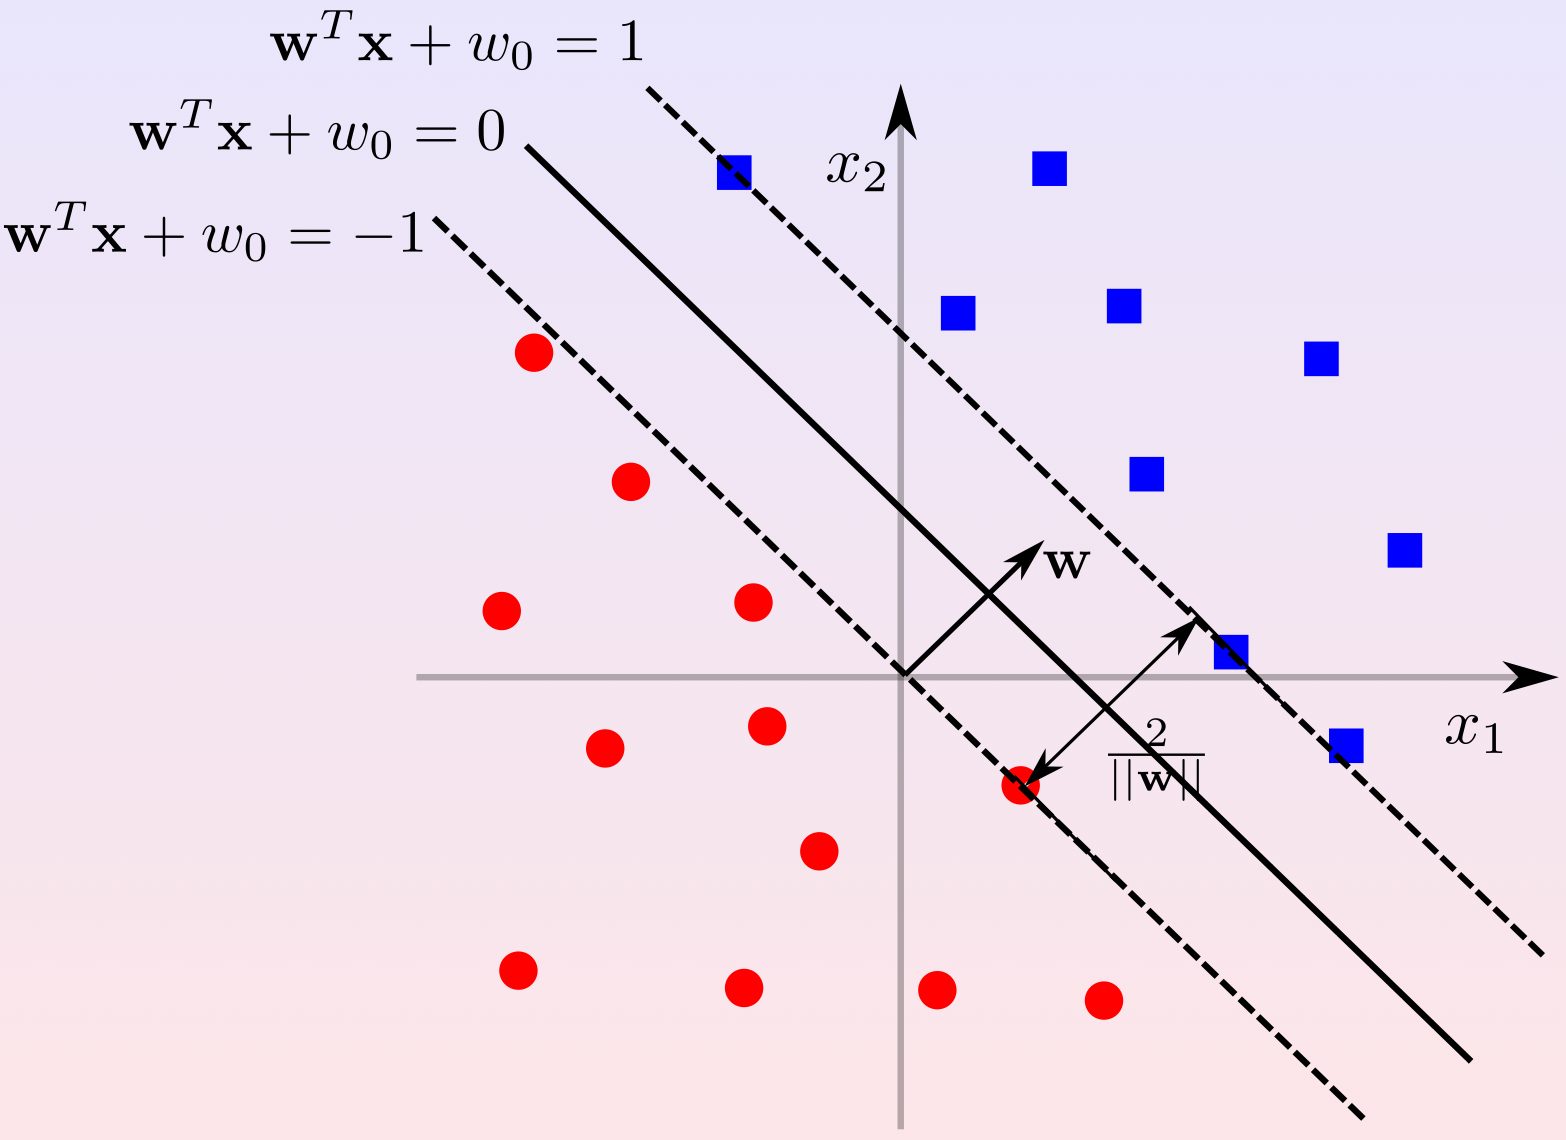
\includegraphics[width=0.7\linewidth]{SVM1}
\end{center}
%
%
%
\section{Hard Margin SVM}
\begin{theorem}[Margin Error Bound]
  Consider the set of decision functions $f(\vect{x})=\sign{\vect{w}^T\vect{x}}$ with $\vert\vert\vect{w}\vert\vert\leq \wedge$ and $\vert\vert\vect{x}\vert\vert\leq R$, for some $R,\wedge>0$. Moreover, let $\rho>0$ and $v$ denote the fraction of training examples with margin smaller than $myfrac{\rho}{\vert\vert\vect{w}\vert\vert}$, referred to as the \textbf{margin error}. \newline
  For all distributions $P$ generating the data, with probability at least $1-\delta$ over the drawing of the $m$ training patterns, and for any $\rho>0$ and $\delta\in(0,1)$, the probability that a test pattern drawn from $P$ will be misclassified is bound from above by:
  \begin{equation}
    v+\sqrt{\frac{c}{m}\left(\frac{R^2\wedge^2}{\rho^2}\ln^2m+\ln\left(\frac{1}{\delta}\right)\right)}
    \label{eq:MarginErrorBound}
  \end{equation}
  where $c$ is a universal constant.
\end{theorem}
What the theorem says is that the probability of test error depends on (among other components):
\begin{itemize}
  \item The number of margin errors $v$, that is examples with margin smaller than $\myfrac{\rho}{\vert\vert\vect{w}\vert\vert}$;
  \item The number of training examples, indeed the error depends on $\myfrac{\ln^2m}{m}$;
  \item The size of the margin, the error depends on $\myfrac{1}{\rho^2}$.
\end{itemize}
Notice that if we are considering the canonical hyperplane, then $\rho=1$ and the problem corresponds to minimizing $\vert\vert\vect{w}\vert\vert$:
\[
  \min\limits_{\vect{w},w_0}\frac{1}{2}\vert\vert\vect{w}\vert\vert^2\quad\text{subject to:}\quad y_i(\vect{w}^T\vect{x}_i+w_0)\geq 1\quad\forall (\vect{x}_i,y_i)\in\mathcal{D}
\]
The constraint guarantees that all points are correctly classified. \newline
Notice that this minimization corresponds to maximizing the (squared) margin. 
%
%
\subsection{Karush-Kuhn-Tucker Approach (KKT)}
This approach starts from the fact that a constrained optimization problem can be addessed by converting it into an unconstrained problem with the same solution. \newline
Let's have a constrained optimization problem in the form:
\[\min\limits_zf(z)\quad\text{subject to:}\quad g_i(z)\geq 0\forall i\]
Now we can introduce a non-negative variable $\alpha_i\geq0$, called Langrange multiplier, for each constraint and rewrite the optimization problem in the form of a Langrangian:
\[\min\limits_z\max\limits_{\alpha\geq0}f(z)-\Sum_i\alpha_ig_i(z)\]
The optimal solutions $z^*$ for this problem are the same as the optimal solutions for the original (constrained) problem:
\begin{itemize}
  \item If for a given $z'$ at least one constraint is not satisfied, i.e., $g_i(z')<0$ for some $i$, then maximizing over $\alpha_i$ leads to an infinite value;
  \item If all constraints are satisfied, i.e., $g_i(z')\geq0\forall i$, then the maximization over the $\vect{\alpha}$ will set all elements of the summation to zero, so that $z'$ is a solution of $\min\limits_zf(z)$.
\end{itemize}
The KKT approach can be used to solve the hard margin SVM constraint by rewriting the problem with a Langrangian as: 
\[L(\vect{w},w_0,\vect{\alpha})=\frac{1}{2}\vert\vert\vect{w}\vert\vert^2-\Sum_{i=1}^m\alpha_i\left(y_i(\vect{w}^T\vect{x}_i+w_0)-1\right)\]
where $m=\vert\mathcal{D}\vert$.
The Langrangian is minimized w.r.t. $\vect{w}, w_0$ and maximized w.r.t. $\alpha_i$. The solution is a saddle point. \newline
Let's then first minimize over $\vect{w}$ and $w_0$:
\[\frac{\partial}{\partial\vect{w}}L(\vect{w},w_0,\vect{\alpha})=0\]
\[\frac{\partial}{\partial\vect{w}}\left(\frac{1}{2}\vert\vert\vect{w}\vert\vert^2-\Sum_{i=1}^m\alpha_i\left(y_i(\vect{w}^T\vect{x}_i+w_0)-1\right)\right)\]

%The constraint we want to specify are:
%\[\forall i
%\begin{cases}
%	y_i-f(x_i)\leq \varepsilon\\
%	f(x_i)-y_i\leq \varepsilon
%\end{cases}
%\]
%And then we want to minimise the normal weight subjects to the constraints:
%\begin{center}
%	$\displaystyle min\frac{\vert\vert w\vert\vert^2}{2} s.t. constraints$
%\end{center}
%We assume that all training instances satisfy the constaints and are therefor within $\varepsilon$: their prediction is out of outmost $\varepsilon$.\newline
%As in classification, we can relax the constraints that all constraints are satisfied by adding slack variables. So if in classification we had:
%\begin{center}
%	$\displaystyle min\frac{\vert\vert w \vert\vert^2}{2} \forall i y_i-f(x_i)\geq 1$
%\end{center}
%Which adding a slack variable becomes:
%\begin{center}
%	$\displaystyle min\frac{\vert\vert w \vert\vert^2}{2} +C\Sum_i\varepsilon_i \forall i y_i-f(x_i)\geq 1-\varepsilon_i$
%\end{center}
%So the regression version becomes:
%\[\forall i
%\begin{cases}
%	y_i-f(x_i)\leq \varepsilon+\epsilon_i\\
%	f(x_i)-y_i\leq \varepsilon+\epsilon^*_i
%\end{cases}
%\]
%With $\epsilon_i, \epsilon^*_i\geq0$. So we need two different slacks. From these we add to the minimise function:
%\begin{center}
%	$\displaystyle min\frac{\vert\vert w\vert\vert^2}{2}+C\Sum_i\epsilon_i\epsilon_i^* s.t. constraints$
%\end{center}
%In this version we do not penalize all example that are outside the queue?\newline
%As for classification we can take the last version and use something to get a Langrangian:
%\begin{center}
%	$\displaystyle \mathcal{L}?\frac{\vert\vertw\vert\vert^2}{2}+C\Sum_i(\epsilon_i+\epsilon?*_i-Sum_i$
%\end{center}
%Meno la somma di qualcosa come $g_i(x)\geq 0$ che diventa quindi:
%\begin{center}
%	$\displaystyle \mathcal{L}?\frac{\vert\vertw\vert\vert^2}{2}+C\Sum_i(\epsilon_i+\epsilon?*_i)-Sum_i\alpha_i(\varepsilon+\epsilon_i-y_i+w^T\phi(x_i)+w_0)$
%\end{center}
%per il primo constraint, e tutto insieme:
%\begin{center}
%	$\displaystyle \mathcal{L}?\frac{\vert\vertw\vert\vert^2}{2}+C\Sum_i(\epsilon_i+\epsilon?*_i-Sum_i\alpha_i(\varepsilon+\epsilon_i-y_i+w^T\phi(x_i)+w_0)-\Sum_i\alpha_i^*(\varepsilon+\epsilon_i^*-y_i+w^T\phi(x_i)+w_0)-\Sum_i\beta_i\epsilon_i-\Sum_i\beta_i^*\epsilon^*_i$
%\end{center}
%Da cui il gradiente diventa:
%\begin{center}
%	$\displaystyle \gradiente_w\mathcal{L}=\frac{2w}{2}-\Sum_i\alpha_i\phi(x_i)+\Sum_i\alpha_i^*\phi(x_i)=0$\\
%	$\displaystyle w=\Sum_i(\alpha^*_i-\alpha_i)\phi(x_i)$
%\end{center}
%Deriviamo ora con rispetto di $w_0$:
%\begin{center}
%	$\displaystyle \frac{\delta\mathcal{L}}{\delta w_0}=-\Sum_i\alpha_i+\Sum_i\alpha_i^*=0$\\
%	$\displaystyle \Sum_i(\alpha_i^*-\alpha_i)=0$
%\end{center}
%Infine deriviamo anche rispetto a $\epsilon_i$ e per $\epsilon_i^*$ :
%\begin{center}
%	$\displaystyle \frac{\delta\mathcal{L}}{\delta \epsilon_i}=C-\alpha_i-\beta_i=0$\\
%	$\displaystyle \frac{\delta\mathcal{L}}{\delta \epsilon_i^*}=C-\alpha_i^*-\beta_i^*=0$\\
%\end{center}
%Ora se le rimettiamo insieme?? otteniamo:
%\begin{center}
%	$\displaystyle \frac{1}{2}\Sum_i(\alpha^*_i-\alpha_i)\phi(x_i))^T(\Sum_j(\alpha_j^*\alpha_j)\phi(x_j))-\Sum_i\alpha_i(\Sum_j(\alpha_j^*-\alpha_j)\phi(x_j))^T\phi(x_i)+\Sum_i\alpha_i^*(\Sum_j(\alpha_j^*-\alpha_j)\phi(x_j))^T\phi(x_i)$
%\end{center}
%Where the first parentesis is $w^T$ and the second is $w$. Now this becomes:
%\begin{center}
%	$\displaystyle =-\frac{1}{2}\Sum_i\Sum_j(\alpha^*_i-\alpha_i)(\alpha_j^*-\alpha_j)\phi(x_i)^T\phi(x_j)$
%\end{center}
%ins{1} \newline
%The result is the one in slide and the function becomes:
%\begin{center}
%	$\displaystyle f(x)=\Sum_i(\alpha_i^*-\alpha_i)\phi(x)^T\phi(x)+w_0$
%\end{center}
%The solution is coming from the dot product between example e chi cazzo ci sta dietro.\newline
%The KKT conditions says that at the point where it's best to maximise or minimise, the sum componente of the langrangian become zero. 
